\documentclass{article}
\usepackage{amsmath}
\usepackage{indentfirst}
\usepackage{graphicx}
\usepackage[a4paper, top=15mm, left=10mm, right=10mm, bottom=15mm]{geometry}

\title{Pattern Recognition Assignment\#4}
\author{61821313 Zihao Wang}
\date{\today}

\linespread{2}
\setlength{\parindent}{2em}

\begin{document}

\maketitle

\section*{Question1}

Here is the decision tree created through information gain

\begin{figure}[htbp]
    \centering
    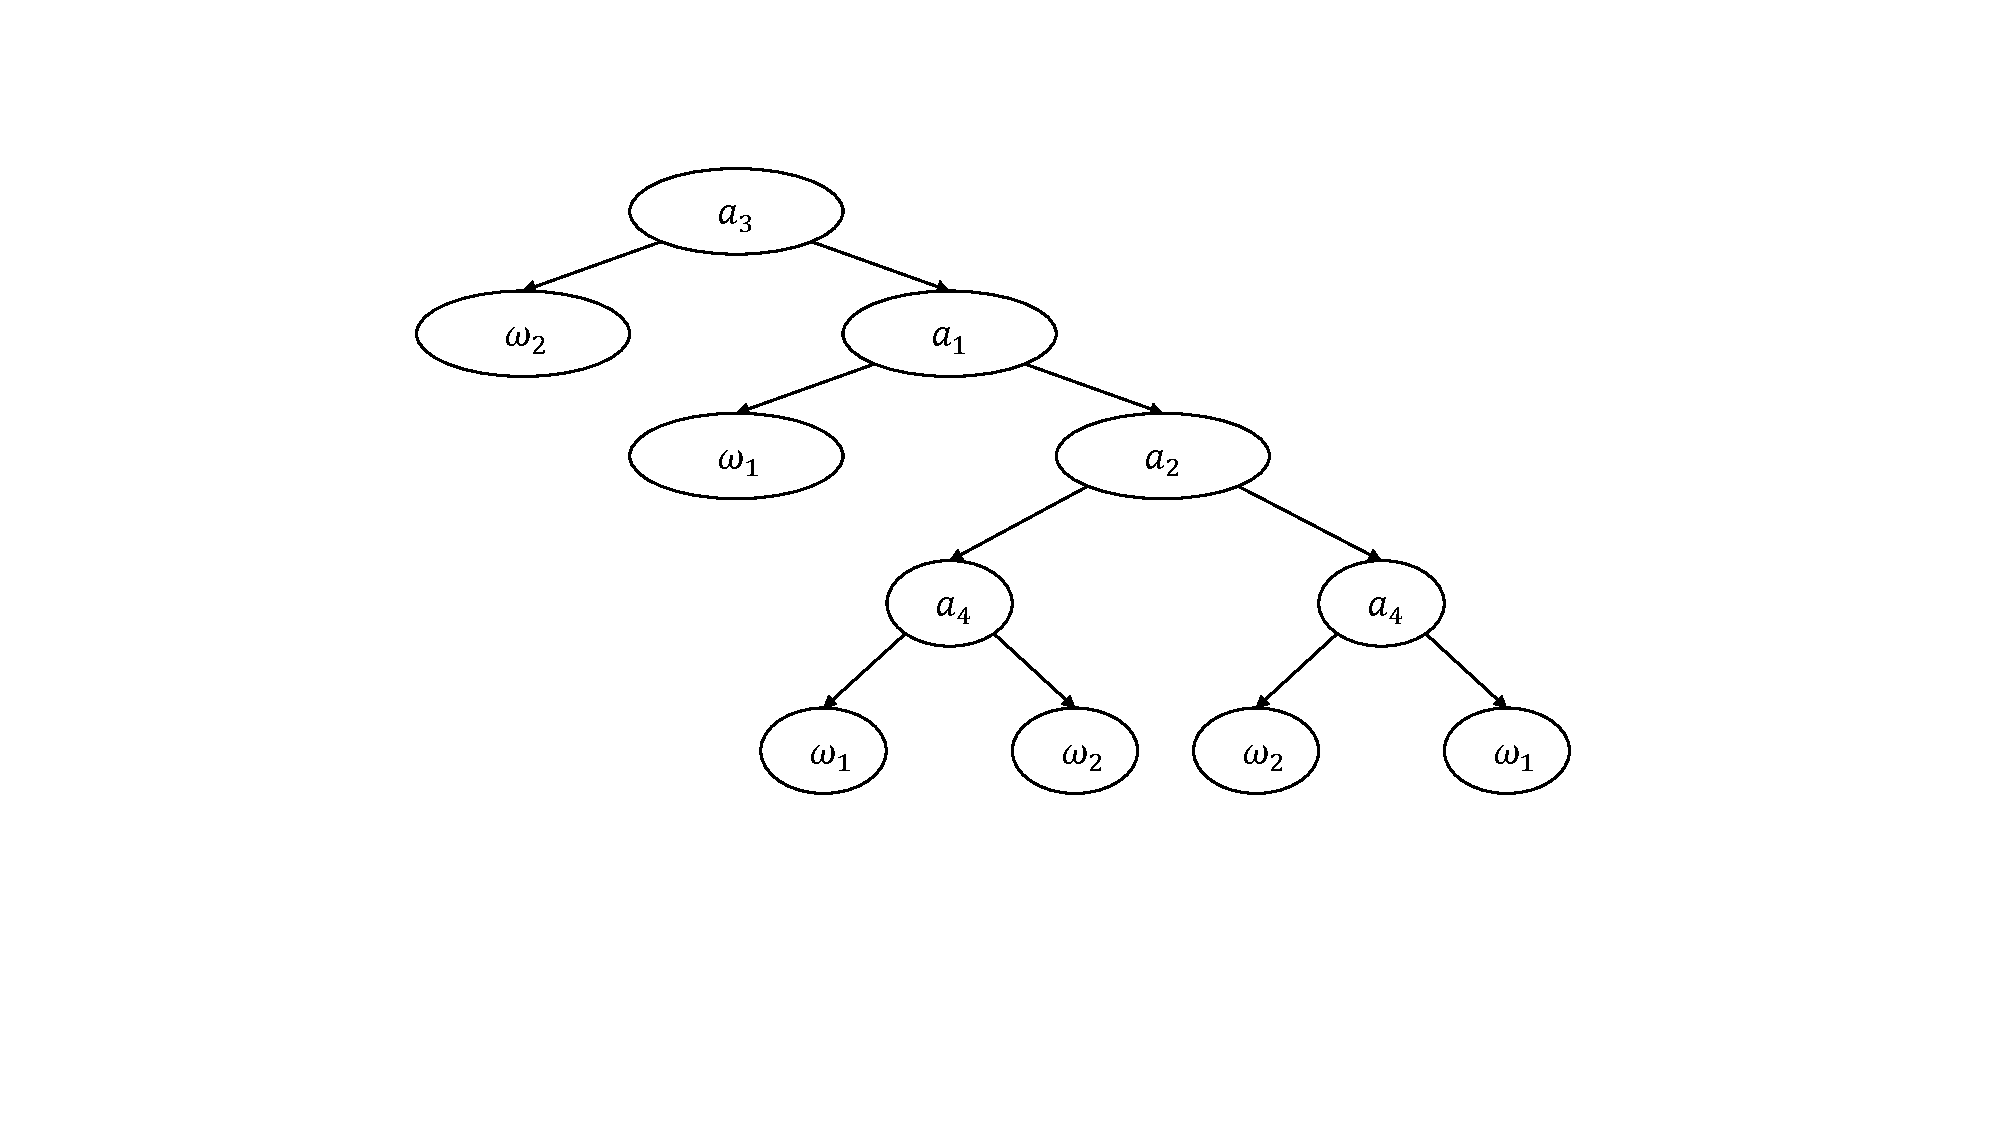
\includegraphics[width=\textwidth, trim=80 150 30 80, clip]{tree.pdf}
    \caption{Decision Tree}
\end{figure}

Where the left child and the right child of a node represent value 0 and 1, respectively

\section*{Question2}

Calculate the hidden layer
\begin{gather*}
net(h_{1}) = w_{11}^{(1)} x_{1} + w_{12}^{(1)} x_{2} = 1.6 \\[3mm]
net(h_{2}) = w_{21}^{(1)} x_{1} + w_{22}^{(1)} x_{2} = 2.8 \\[3mm]
h_{1} = f(net(h_{1})) = 0.8320 \\[3mm]
h_{2} = f(net(h_{2})) = 0.9427
\end{gather*}

Calculate the output layer
\begin{gather*}
net(o) = w_{11}^{(2)} h_{1} + w_{12}^{(2)} h_{2} = 1.1591 \\[3mm]
o = f(net(o)) = 0.7612
\end{gather*}

Use the square loss as the loss function
\begin{equation*}
\ell = \frac{1}{2} (t - o)^{2}
\end{equation*}

Calculate the dirivative of the net activation of output layer
\begin{gather*}
\frac{\partial \ell}{\partial o} = o - t = -0.2388 \\[3mm]
\frac{\partial o}{\partial net(o)} = o(1 - o) = 0.1818 \\[3mm]
\frac{\partial \ell}{\partial net(o)} = \frac{\partial \ell}{\partial o} 
\frac{\partial o}{\partial net(o)} = -0.0434
\end{gather*}

Calculate the dirivative of the hidden-to-output layer weights and the hidden layer
\begin{gather*}
\frac{\partial net(o)}{\partial w_{11}^{(2)}} = h_{1} = 0.8320 \qquad
\frac{\partial \ell}{\partial w_{11}^{(2)}} = \frac{\partial \ell}{\partial net(o)} 
\frac{\partial net(o)}{\partial w_{11}^{(2)}} = -0.0361\\[3mm]
\frac{\partial net(o)}{\partial w_{12}^{(2)}} = h_{2} = 0.9427 \qquad
\frac{\partial \ell}{\partial w_{12}^{(2)}} = \frac{\partial \ell}{\partial net(o)} 
\frac{\partial net(o)}{\partial w_{12}^{(2)}} = -0.0409 \\[3mm]
\frac{\partial net(o)}{\partial h_{1}} = w_{11}^{(2)} = 0.6 \qquad
\frac{\partial \ell}{\partial h_{1}} = \frac{\partial \ell}{\partial net(o)} 
\frac{\partial net(o)}{\partial h_{1}} = -0.0260 \\[3mm]
\frac{\partial net(o)}{\partial h_{2}} = w_{12}^{(2)} = 0.7 \qquad
\frac{\partial \ell}{\partial h_{2}} = \frac{\partial \ell}{\partial net(o)} 
\frac{\partial net(o)}{\partial h_{2}} = -0.0304
\end{gather*}

Calculate the dirivative of the net activation of hidden layer
\begin{gather*}
\frac{\partial h_{1}}{\partial net(h_{1})} = h_{1}(1 - h_{1}) = 0.1398 \\[3mm]
\frac{\partial h_{2}}{\partial net(h_{2})} = h_{2}(1 - h_{2}) = 0.0540 \\[3mm]
\frac{\partial \ell}{\partial net(h_{1})} = \frac{\partial \ell}{\partial h_{1}} 
\frac{\partial h_{1}}{\partial net(h_{1})} = -3.6348 \times 10^{-3} \\[3mm]
\frac{\partial \ell}{\partial net(h_{2})} = \frac{\partial \ell}{\partial h_{2}} 
\frac{\partial h_{2}}{\partial net(h_{2})} = -1.6416 \times 10^{-3}
\end{gather*}

Calculate the dirivative of the input-to-hidden layer weights
\begin{gather*}
\frac{\partial net(h_{1})}{\partial w_{11}^{(1)}} = x_{1} = 2 \qquad
\frac{\partial \ell}{\partial w_{11}^{(1)}} = \frac{\partial \ell}{\partial net(h_{1})} 
\frac{\partial net(h_{1})}{\partial w_{11}^{(1)}} = -7.2696 \times 10^{-3} \\[3mm]
\frac{\partial net(h_{1})}{\partial w_{12}^{(1)}} = x_{2} = 4 \qquad
\frac{\partial \ell}{\partial w_{12}^{(1)}} = \frac{\partial \ell}{\partial net(h_{1})} 
\frac{\partial net(h_{1})}{\partial w_{12}^{(1)}} = -1.4539 \times 10^{-2} \\[3mm]
\frac{\partial net(h_{2})}{\partial w_{21}^{(1)}} = x_{1} = 2 \qquad
\frac{\partial \ell}{\partial w_{11}^{(1)}} = \frac{\partial \ell}{\partial net(h_{2})} 
\frac{\partial net(h_{2})}{\partial w_{21}^{(1)}} = -3.2832 \times 10^{-3} \\[3mm]
\frac{\partial net(h_{2})}{\partial w_{22}^{(1)}} = x_{2} = 4 \qquad
\frac{\partial \ell}{\partial w_{22}^{(1)}} = \frac{\partial \ell}{\partial net(h_{2})} 
\frac{\partial net(h_{2})}{\partial w_{22}^{(1)}} = -6.5664 \times 10^{-3}
\end{gather*}

Update the layer weights $\boldsymbol{w}$ through the dirivative
\begin{equation*}
\boldsymbol{w} \leftarrow \boldsymbol{w} - \eta \frac{\partial \ell}{\partial \boldsymbol{w}}
\end{equation*}

The resulting model $\boldsymbol{w}$ after training is
\begin{equation*}
\boldsymbol{w} = \{ 0.2073,\ 0.3145,\ 0.4033,\ 0.5066,\ 0.6361,\ 0.7409 \}
\end{equation*}

\end{document}